\documentclass[11pt, letterpaper]{article}
% Phase 12A — UG Summer Research Internship Final Report
% Format follows the CUHK CSE sample final report: single column, Times
% serif, 1-inch margins, 1.5 line spacing, arabic section numbers, cover
% page with university header, table of contents, author-year citations.

\usepackage{amsmath,amssymb,amsfonts}
\usepackage{graphicx}
\usepackage{textcomp}
\usepackage{xcolor}
\usepackage{booktabs}
\usepackage{tabularx}
\usepackage{caption}
% More breathing room between table caption and the table body;
% table captions indented 3cm on each side (same as figure captions)
\captionsetup[table]{skip=14pt, margin=3cm}
% Figure captions indented 3cm on each side
\captionsetup[figure]{margin=3cm}
\usepackage{tikz}
\usetikzlibrary{positioning,arrows.meta,shapes.geometric,calc}
% Times New Roman (system font, XeLaTeX)
\usepackage{fontspec}
\setmainfont{Times New Roman}
% Monospace for code identifiers (fontspec: \ttdefault override is TU-incompatible)
\setmonofont{Courier New}
% Margins: all sides 2.04cm (1in minus 0.5cm), then left/right reduced
% another 0.5cm -> 1.54cm; top/bottom stay at 2.04cm
\usepackage[left=1.54cm, right=1.54cm, top=2.04cm, bottom=2.04cm]{geometry}
\usepackage{setspace}
\onehalfspacing
% Numbered citations: [1], [2], ... in text and reference list
\usepackage[numbers,square,comma]{natbib}
\setcitestyle{square,comma,numbers}
\usepackage{fancyhdr}
\pagestyle{fancy}
\fancyhf{}
\fancyfoot[C]{\thepage}
\renewcommand{\headrulewidth}{0pt}
\usepackage{hyperref}
\hypersetup{colorlinks=true, linkcolor=black, urlcolor=blue, citecolor=blue,
    pageanchor=false}
% Allow LaTeX to stretch glue slightly to avoid marginal overfull hboxes.
\setlength{\emergencystretch}{2em}
\def\BibTeX{{\rm B\kern-.05em{\sc i\kern-.025em b}\kern-.08em
    T\kern-.1667em\lower.7ex\hbox{E}\kern-.125emX}}

\begin{document}

% ================= Cover page =================
\begin{titlepage}
\thispagestyle{empty}
\centering
{\large \textbf{The Chinese University of Hong Kong}\par}
\vspace{0.3cm}
{\normalsize Department of Information Engineering, Faculty of Engineering\par}
\vspace{0.4cm}
\rule{\textwidth}{0.6pt}
\vspace{1.2cm}
{\Large \textbf{Summer Research Project}\par}
\vspace{1.4cm}
{\LARGE \textbf{Heterogeneous Bipartite Graph Neural Networks for GUI Structure Error Correction}\par}
\vspace{0.5cm}
{\large A Post-Correction Framework for Lightweight Vision-Language Models\par}
\vspace{2.5cm}
{\normalsize \textbf{Author:}\par}
{\large Xie Licheng (Alex)\par}
{\normalsize 1155246441\par}
\vspace{1.2cm}
{\normalsize \textbf{Supervisor:}\par}
{\large Prof.\ Wing Cheong Lau (IE)\par}
\vfill
{\normalsize August 2026\par}
\end{titlepage}

\tableofcontents
\newpage

\begin{abstract}
Computer programs that ``look at'' a phone screen (assistive tools for
visually impaired users, automated UI testers, and software agents) all
need to know what is on the screen and where. Small vision-language models
(VLMs) are attractive for running such tasks directly on a phone because they
are fast and memory-efficient, but they make mistakes: they miss 10--30\% of
the visible interface elements, and the bounding boxes they draw around the
elements they do find are often misaligned with reality. This report presents
a post-correction framework that fixes these mistakes without retraining the
VLM or adding a second detector. The underlying assumption is that
well-designed interfaces obey spatial rules: elements align, sit inside
containers, and follow consistent spacing. We encode these rules as a
heterogeneous bipartite graph: one set of nodes for the detected elements,
one set for the spatial constraints among them, and edges only between the
two sets. A GraphSAGE network passes messages along this graph so that every
element's prediction is informed by its spatial neighbours, then predicts
per-element coordinate corrections, flags violated constraints, scores
whether each detection is real or hallucinated, and proposes elements the
VLM missed entirely. On the RICO dataset (real Android screenshots), the
model detects violated constraints at 90--94\% accuracy and, when a large
fraction of elements is missing, completes the layout with up to 56\% better
IoU than a nearest-neighbor baseline. End-to-end on 200 real screenshots with
a Qwen3-VL Flash front end, the corrected pipeline recovers 106 previously
missed elements, raising F1 by 2.0 points and recall by 2.2 points. The
correction module runs after the VLM, does not modify the underlying model,
and adds less than one millisecond of inference per screenshot.
\end{abstract}

\section{Introduction}
To understand a smartphone interface, a program must first
answer a basic question: \emph{what is on this screen, and where is it?}
Every application (from screen readers for visually impaired users, to
automated UI testers, to software agents that operate a phone on a user's
behalf) depends on accurate knowledge of the interface elements (buttons,
text fields, icons, images) and their positions.

\subsection{Why Lightweight Vision-Language Models}
Vision-language models (VLMs) are neural networks that can describe images in
natural language and, given a screenshot, can list the interface elements and
their bounding boxes. Large VLMs with 7 billion parameters or more are quite
accurate at this task, but they are too slow and too memory-hungry to run on a
phone. Lightweight VLMs under 3 billion parameters (such as Qwen3-VL Flash
\cite{bai2023qwen} and MiniMax-VL-01) are fast enough for on-device use, which
makes them attractive for real-time applications.

\subsection{Two Systematic Failure Modes}
Evaluation on real screenshots shows that lightweight VLMs make two
kinds of mistakes:

\begin{itemize}
\item \textbf{Element omission.} 10--30\% of the visible elements are never
reported. Small icons, dividers, and nested containers are missed most often.
\item \textbf{Misalignment.} The bounding boxes around detected elements can
deviate by tens of pixels from where the element actually is, which breaks
downstream reasoning about layout.
\end{itemize}

These are not random glitches; they are systematic consequences of
compressing a large model into a small one. The natural response, training a
bigger model, is precisely what on-device constraints forbid.

\subsection{Our Approach in One Paragraph}
Early experiments shaped this design. We first attempted to correct
coordinates directly, training an MLP on per-element features. The results
were consistently poor: on simulated Gaussian noise the model never beat the
no-op baseline, and on real VLM output (Qwen3-VL Plus and Flash) the
positional errors were already small enough that there was little to correct.
A local LLaVA-7B model produced too few detections per screenshot for the
graph to carry useful structure. These failures pointed to a common cause:
single-element features carried too little context for coordinate
prediction, regardless of how the regressor was trained.

The alternative explored in this report is to exploit structure. GUI
screenshots are laid out according to spatial rules such as alignment,
containment, spacing, and grid membership. These rules are independent
evidence that a VLM looking at pixels alone cannot use: if every element in
a row is left-aligned except one, the odd one out is probably misplaced,
regardless of what the pixels look like. We formalize these rules as a graph:
element nodes on one side, constraint nodes on the other, and edges connecting
an element to every constraint it participates in. A graph neural network
(GraphSAGE) then reasons over this structure and outputs corrected
coordinates, violated constraints, per-element confidence, and (for the
omission problem) entirely new element proposals. Because the correction
runs after the VLM, it does not modify the underlying model: the same
correction network works behind any VLM that outputs elements with bounding
boxes.

The rest of this report is organized as follows. Section~II summarizes
existing solutions and their limitations. Section~III describes the proposed
method in detail. Section~IV presents experiments and results. Section~V
discusses limitations and future work, and Section~VI concludes.

\section{Existing Solutions and Their Limitations}
\subsection{Fine-Tuning Larger Models}
The most direct remedy for VLM mistakes is to fine-tune a larger VLM (7B+) on
GUI data, or to fine-tune the lightweight model on domain-specific screenshots.
This improves accuracy but has two costs: it requires labeled GUI data, and
(more fundamentally for the on-device use case) the improved model is
larger, slower, or both. Fine-tuning also bakes in a specific VLM; swapping
the front-end model means retraining everything.

\subsection{Object-Detector Cascades}
A different approach adds a dedicated object detector (for example, a DETR
\cite{carion2020detr} model) in front of or alongside the VLM. Detectors are
accurate but add a second network to run on-device, increasing latency and
memory, and require their own training data. The cascade approach treats the
GUI as a generic object-detection problem, discarding the strong spatial
structure that all well-designed interfaces share.

\subsection{Generative Layout Models}
LayoutGAN \cite{li2019layoutgan} and LayoutTransformer
\cite{gupta2021layouttransformer} learn layout priors and can \emph{generate}
new layouts. They are generative: given random noise or partial structure,
Our problem is different: we receive a
noisy layout and must \emph{repair} it, but the idea of a learned layout
prior is shared. We make the prior explicit and interpretable (ten spatial
constraint types) rather than implicit in a generative model.

\subsection{Why a Correction Network}
The framework proposed here differs from the approaches above in one
respect: it never generates pixels or detections from scratch, and it never
modifies the VLM. It \emph{post-processes} the VLM's noisy output using
structural reasoning. This choice was motivated by the on-device constraint:
the VLM is the expensive component, and any fix that forces a larger model or
an additional detector undoes the reason for using a lightweight VLM in the
first place. Post-processing keeps the VLM unchanged, adds a small graph
network (57K parameters), and works with any VLM that outputs a list of
elements with bounding boxes. The trade-off is that the correction is limited
by what the VLM initially detects; elements missed entirely can only be
recovered through the completion head, which is evaluated in Section~IV.

\section{Proposed Method}
\subsection{Overview}
The pipeline is shown in Fig.~\ref{fig:pipeline}. A screenshot is fed to a
lightweight VLM, which produces a noisy JSON list of detected elements. We
convert that list into a heterogeneous bipartite graph, run two hops of
GraphSAGE message passing, and read out corrections from four prediction
heads. The output is a corrected JSON with refined boxes, new proposals for
missed elements, and per-element reliability scores.

\begin{figure}[htbp]
\centering
\resizebox{\textwidth}{!}{%
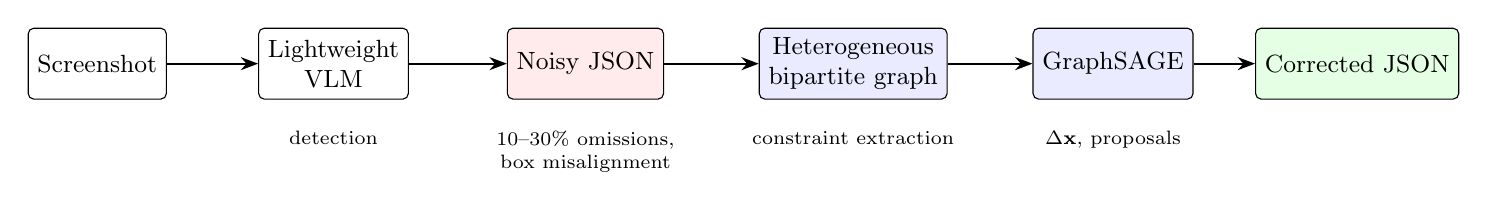
\begin{tikzpicture}[
    box/.style={draw, rounded corners=2pt, align=center, minimum height=0.9cm,
                font=\small},
    arr/.style={-{Stealth[length=2.2mm]}, thick},
    scale=1.0, transform shape]
  \node[box] (shot) at (0,0) {Screenshot};
  \node[box] (vlm) at (3.0,0) {Lightweight\\VLM};
  \node[box, fill=red!8] (noisy) at (6.2,0) {Noisy JSON};
  \node[box, fill=blue!8] (graph) at (9.6,0) {Heterogeneous\\bipartite graph};
  \node[box, fill=blue!8] (gnn) at (12.9,0) {GraphSAGE};
  \node[box, fill=green!10] (out) at (16.0,0) {Corrected JSON};
  \draw[arr] (shot) -- (vlm);
  \draw[arr] (vlm) -- (noisy);
  \draw[arr] (noisy) -- (graph);
  \draw[arr] (graph) -- (gnn);
  \draw[arr] (gnn) -- (out);
  \node[font=\scriptsize, below=0.28cm of vlm] {detection};
  \node[font=\scriptsize, align=center, below=0.28cm of noisy] {10--30\% omissions,\\box misalignment};
  \node[font=\scriptsize, below=0.28cm of graph] {constraint extraction};
  \node[font=\scriptsize, below=0.28cm of gnn] {$\Delta\mathbf{x}$, proposals};
\end{tikzpicture}}
\caption{Pipeline overview: screenshot, lightweight VLM, noisy element
list, bipartite graph, GraphSAGE, corrected JSON.}
\label{fig:pipeline}
\end{figure}

\subsection{Formalizing a Screenshot as a Graph}
\subsubsection{Elements}
\sloppy
Let a screenshot yield $N$ detected elements
$\mathcal{E}=\{e_i\}_{i=1}^{N}$, each with a normalized bounding box
$\mathbf{b}_i=(x_1^{(i)},y_1^{(i)},x_2^{(i)},y_2^{(i)})\in[0,1]^4$ (the box
coordinates, scaled so the image is a unit square) and a type label
$t_i\in\mathcal{T}$ from the element taxonomy (button, text field, icon,
image, etc.).

\subsubsection{Spatial Constraints}
From these elements we extract $M$ spatial constraints
$\mathcal{C}=\{c_j\}_{j=1}^{M}$, where each constraint is a typed relationship
between elements. Table~\ref{tab:constraints} lists the ten constraint types.
Each constraint $c_j$ has a type $\tau_j$, a source index set
$S_j\subseteq\{1,\dots,N\}$, and a target index set
$T_j\subseteq\{1,\dots,N\}$; the constraint exists when its predicate
$P_\tau(\mathbf{b}_{S_j},\mathbf{b}_{T_j})$ holds within a tolerance
$\varepsilon$.

\begin{table}[htbp]
\caption{The ten spatial constraint types extracted from a layout.}
\label{tab:constraints}
\centering
\begin{tabularx}{\textwidth}{lXX}
\toprule
\textbf{Type} & \textbf{Predicate} & \textbf{Example} \\
\midrule
\texttt{ALIGN\_LEFT} & $|x_1-x_1'|<\varepsilon$ & Buttons share a left edge \\
\texttt{ALIGN\_RIGHT} & $|x_2-x_2'|<\varepsilon$ & Right edges aligned \\
\texttt{ALIGN\_TOP} & $|y_1-y_1'|<\varepsilon$ & Top edges aligned \\
\texttt{ALIGN\_BOTTOM} & $|y_2-y_2'|<\varepsilon$ & Bottom edges aligned \\
\texttt{CENTER\_X} & center-distance $<\varepsilon$ & Horizontally centered \\
\texttt{CENTER\_Y} & center-distance $<\varepsilon$ & Vertically centered \\
\texttt{SPACING} & consistent gaps & Evenly spaced list items \\
\texttt{CONTAINMENT} & one box inside another & Icon inside a container \\
\texttt{GRID} & row/column membership & Grid layout detection \\
\texttt{SAME\_SIZE} & similar widths/heights & Uniform card sizes \\
\bottomrule
\end{tabularx}
\end{table}

\subsubsection{The Bipartite Graph}
The GUI structure is a \emph{heterogeneous bipartite graph}
\begin{equation}
G=(\mathcal{V},\mathcal{E}_{\text{edge}},\phi,\psi),
\label{eq:graph}
\end{equation}
where $\mathcal{V}=\mathcal{E}\cup\mathcal{C}$ is the node set, partitioned
into element nodes $V_e$ ($|V_e|=N$) and constraint nodes $V_c$ ($|V_c|=M$);
$\phi:\mathcal{V}\to\{0,1\}$ labels each node's partition; edges exist only
between partitions; an edge $(e_i,c_j)$ connects element $e_i$ to
constraint $c_j$ iff $e_i\in S_j\cup T_j$; and $\psi$ weights each edge by
the normalized distance between the element and the constraint's subspace.
There are no element--element or constraint--constraint edges. Fig.~\ref{fig:arch}
illustrates the structure.

\begin{figure}[htbp]
\centering
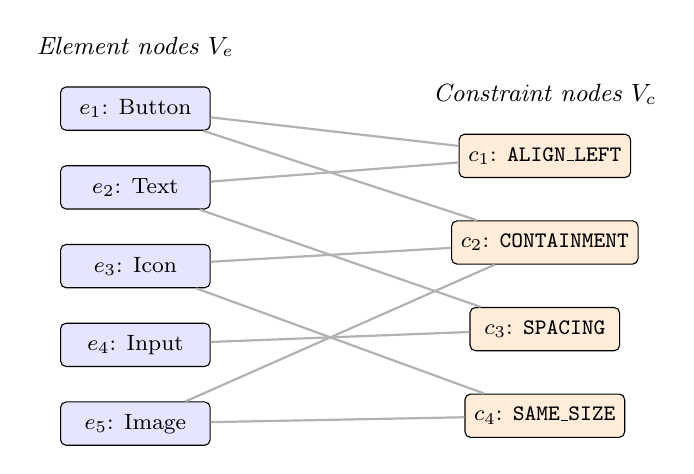
\begin{tikzpicture}[
    elem/.style={draw, rounded corners=2pt, fill=blue!10, minimum width=1.9cm,
                 minimum height=0.55cm, font=\footnotesize},
    cons/.style={draw, rounded corners=2pt, fill=orange!15, minimum width=1.9cm,
                 minimum height=0.55cm, font=\footnotesize},
    edg/.style={gray!60, thick},
    scale=1.0, transform shape]
  % element nodes (left)
  \node[elem] (e1) at (0,2.6) {$e_1$: Button};
  \node[elem] (e2) at (0,1.6) {$e_2$: Text};
  \node[elem] (e3) at (0,0.6) {$e_3$: Icon};
  \node[elem] (e4) at (0,-0.4) {$e_4$: Input};
  \node[elem] (e5) at (0,-1.4) {$e_5$: Image};
  % constraint nodes (right)
  \node[cons] (c1) at (5.2,2.0) {$c_1$: \texttt{ALIGN\_LEFT}};
  \node[cons] (c2) at (5.2,0.9) {$c_2$: \texttt{CONTAINMENT}};
  \node[cons] (c3) at (5.2,-0.2) {$c_3$: \texttt{SPACING}};
  \node[cons] (c4) at (5.2,-1.3) {$c_4$: \texttt{SAME\_SIZE}};
  % edges: only cross-partition
  \draw[edg] (e1) -- (c1);
  \draw[edg] (e1) -- (c2);
  \draw[edg] (e2) -- (c1);
  \draw[edg] (e2) -- (c3);
  \draw[edg] (e3) -- (c2);
  \draw[edg] (e3) -- (c4);
  \draw[edg] (e4) -- (c3);
  \draw[edg] (e5) -- (c4);
  \draw[edg] (e5) -- (c2);
  % partition labels
  \node[font=\small\itshape, above=0.25cm of e1] {Element nodes $V_e$};
  \node[font=\small\itshape, above=0.25cm of c1] {Constraint nodes $V_c$};
\end{tikzpicture}
\caption{Heterogeneous bipartite graph: element nodes (left) connect only to
constraint nodes (right). No two elements are ever connected directly; they
communicate through shared constraints.}
\label{fig:arch}
\end{figure}

\subsection{Message Passing}
A graph neural network propagates information along the edges. We use two
alternating hops of GraphSAGE convolution \cite{hamilton2017sage}, which
aggregates neighboring features with a mean operation.

\subsubsection{Hop 1: Element to Constraint}
Each constraint node collects information from the elements it involves:
\begin{equation}
\mathbf{h}_{c_j}^{(1)}=\sigma\!\left(\mathbf{W}_1\cdot
\operatorname{MEAN}\!\left(\left\{\mathbf{h}_{e_i}^{(0)}:
(e_i,c_j)\in\mathcal{E}_{\text{edge}}\right\}\right)+\mathbf{b}_1\right),
\label{eq:hop1}
\end{equation}
where $\mathbf{h}_{e_i}^{(0)}$ is the initial element feature vector and
$\sigma$ is the ReLU activation. Intuitively, the constraint node now
``knows'' the aggregate state of the elements that share it.

\subsubsection{Hop 2: Constraint to Element}
Each element node collects the updated constraint states back:
\begin{equation}
\mathbf{h}_{e_i}^{(2)}=\sigma\!\left(\mathbf{W}_2\cdot
\operatorname{MEAN}\!\left(\left\{\mathbf{h}_{c_j}^{(1)}:
(e_i,c_j)\in\mathcal{E}_{\text{edge}}\right\}\right)+\mathbf{b}_2\right).
\label{eq:hop2}
\end{equation}
After this hop, every element's representation carries information from all
elements that share a constraint with it, its ``spatial neighbourhood.''
Elements that share no constraint never exchange messages, which keeps the
inductive bias strong and computation local.

\subsection{Node Features}
Each element's initial feature $\mathbf{h}_{e_i}^{(0)}$ is 5-dimensional: the
four normalized box coordinates plus the normalized area
$a_i=(x_2-x_1)(y_2-y_1)$. An optional frozen visual feature
$\mathbf{v}_i\in\mathbb{R}^{d_v}$ (192-d ViT-Tiny or 768-d
DINOv2 \cite{oquab2024dinov2}) can be concatenated. Constraint node features
embed the constraint type as a 10-d one-hot vector plus spatial statistics of
the participating elements (mean pairwise distance, containment overlap
ratio, alignment residual).

\subsection{Four Prediction Heads}
After message passing, four heads read out the result. The total training
objective is a weighted sum
\begin{equation}
\mathcal{L}=w_c\,\mathcal{L}_{\text{coord}}+w_v\,\mathcal{L}_{\text{vio}}
+w_e\,\mathcal{L}_{\text{exist}}+w_p\,\mathcal{L}_{\text{prop}},
\label{eq:loss}
\end{equation}
with default weights $w_c{=}1.0$, $w_v{=}0.5$, $w_e{=}0.5$, $w_p{=}0.5$.

\subsubsection{Coordinate Correction}
The first head predicts a per-element delta vector
$\Delta\mathbf{x}_i=\operatorname{MLP}_{\text{coord}}(\mathbf{h}_{e_i}^{(2)})$,
the amount by which the VLM's box should move, optimized with a smooth
L1 loss:
\begin{equation}
\mathcal{L}_{\text{coord}}=\frac{1}{N}\sum_{i=1}^{N}
\operatorname{smooth}_{L_1}(\Delta\mathbf{x}_i-\Delta\mathbf{x}_i^*),
\label{eq:lcoord}
\end{equation}
where $\Delta\mathbf{x}_i^*$ is the ground-truth correction.

\subsubsection{Violation Detection}
The second head classifies whether each constraint is violated (broken), with
$\hat{v}_j=\sigma(\operatorname{MLP}_{\text{vio}}(\mathbf{h}_{c_j}^{(1)}))$:
\begin{equation}
\mathcal{L}_{\text{vio}}=-\frac{1}{M}\sum_{j=1}^{M}\bigl[
v_j^*\log\hat{v}_j+(1-v_j^*)\log(1-\hat{v}_j)\bigr],
\label{eq:lvio}
\end{equation}
where $v_j^*\in\{0,1\}$ indicates whether constraint $c_j$ is genuinely
violated in the ground-truth layout. This head is what makes the model
``understand'' layout rules: it must learn what a broken alignment or
containment looks like from the graph alone.

\subsubsection{Existence Scoring}
The third head scores whether each detected element is real or hallucinated,
predicting $\hat{e}_i$ with a binary classifier on the element embedding and
training with binary cross-entropy:
\begin{equation}
\mathcal{L}_{\text{exist}}=-\frac{1}{N}\sum_{i=1}^{N}\bigl[
e_i^*\log\hat{e}_i+(1-e_i^*)\log(1-\hat{e}_i)\bigr],
\label{eq:lexist}
\end{equation}
where $e_i^*$ is the ground-truth existence label. Downstream, this score can
filter false positives or rank elements by reliability.

\subsubsection{Element Completion}
The fourth head, the one that addresses the omission problem, proposes
\emph{missing} elements. During training, we randomly drop a fraction
$\rho\in[0.2,0.8]$ of the ground-truth elements. A constraint that referenced
a dropped element now has a ``hole'' (a dangling edge), which is exactly the
signature a missing element leaves in the graph. The head predicts the
missing element's box and type from the aggregated constraint embedding:
\begin{equation}
\hat{\mathbf{b}}_k,\hat{t}_k=
\operatorname{MLP}_{\text{proposal}}(\mathbf{h}_{c_j}^{(1)}),
\qquad
\mathcal{L}_{\text{prop}}=\frac{1}{K}\sum_{k=1}^{K}\bigl[
\mathcal{L}_{\text{IoU}}(\hat{\mathbf{b}}_k,\mathbf{b}_k^*)
+\alpha\,\mathrm{CE}(\hat{t}_k,t_k^*)\bigr],
\label{eq:lprop}
\end{equation}
where $K$ is the number of violated constraints with a missing target and
$\mathcal{L}_{\text{IoU}}$ is the IoU-based box loss. Note that the training
signal is derived purely by masking ground-truth layouts; the completion
head is \emph{self-supervised}: it needs no additional human annotation.

\section{Experiments and Results}
\subsection{Experimental Setup}
All models use AdamW with cosine annealing, a 128-d hidden dimension, and
two-layer bipartite GraphSAGE, trained with 5 random seeds where reported.
We evaluate on the RICO dataset \cite{dek.a17rico} (real Android screenshots)
and ScreenSpot \cite{cheng2024screenspot}. Implementation uses
PyTorch \cite{paszke2019pytorch}, PyTorch Geometric \cite{fey2019pyg},
NumPy \cite{harris2020numpy}, SciPy \cite{virtanen2020scipy}, and
Matplotlib \cite{hunter2007matplotlib}; the front-end VLM is
Qwen3-VL Flash \cite{bai2023qwen}.

\subsection{Constraint-Type Ablation}
Which spatial rules matter most? We ablate the ten constraint types on the
violation-detection task (Table~\ref{tab:ablation}, Fig.~\ref{fig:ablation}).
Removing containment causes the largest accuracy drop ($-1.9$pp), confirming
that parent--child containment is the strongest structural signal. Removing
\emph{all} alignment types \emph{increases} accuracy to 93.9\%: with far
fewer constraints per graph, the remaining violations are easier to
classify. Keeping only alignment types hurts most ($-3.0$pp): alignment alone
cannot support violation detection.

\begin{table}[htbp]
\caption{Constraint-type ablation on violation detection (n=500, drop=0.6).}
\label{tab:ablation}
\centering
\begin{tabularx}{\textwidth}{Xc}
\toprule
\textbf{Constraint set} & \textbf{Violation acc.} \\
\midrule
All 10 types (control) & \textbf{0.908} \\
\texttt{CONTAINMENT} & 0.889 ($-1.9$pp) \\
\texttt{SPACING} & 0.903 ($-0.5$pp) \\
\texttt{GRID} & 0.916 ($+0.8$pp) \\
Remove all \texttt{ALIGNMENT} & 0.939 ($+3.1$pp) \\
Only \texttt{ALIGNMENT} & 0.878 ($-3.0$pp) \\
\bottomrule
\end{tabularx}
\end{table}

\begin{figure}[htbp]
\centering
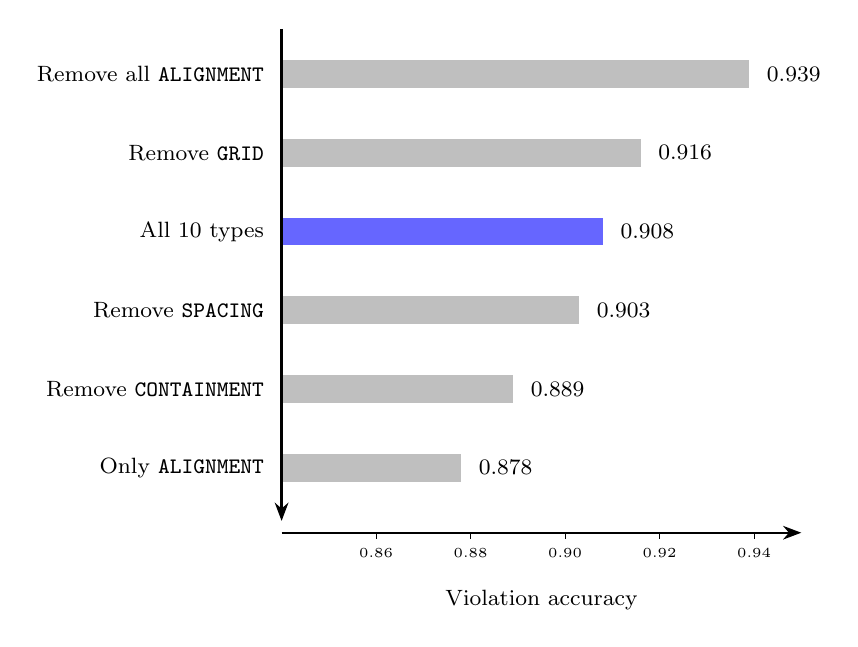
\begin{tikzpicture}[scale=1.0, transform shape]
  % horizontal bars: length = (value - 0.84) * 60 cm
  \def\sc{60}
  \def\base{0.0}
  % y positions for 6 rows (top to bottom), bar height 0.35; sorted desc by value
  % Remove all ALIGNMENT 0.939 -> 5.94cm
  \fill[gray!50] (\base,5.0) rectangle ({(\base+(0.939-0.84)*\sc)},5.35);
  \node[anchor=east, font=\footnotesize] at (\base-0.1,5.175) {Remove all \texttt{ALIGNMENT}};
  \node[font=\footnotesize, anchor=west] at ({(\base+(0.939-0.84)*\sc+0.1)},5.175) {0.939};
  % Remove GRID 0.916 -> 4.56cm
  \fill[gray!50] (\base,4.0) rectangle ({(\base+(0.916-0.84)*\sc)},4.35);
  \node[anchor=east, font=\footnotesize] at (\base-0.1,4.175) {Remove \texttt{GRID}};
  \node[font=\footnotesize, anchor=west] at ({(\base+(0.916-0.84)*\sc+0.1)},4.175) {0.916};
  % All 10 types (control) 0.908 -> 4.08cm
  \fill[blue!60] (\base,3.0) rectangle ({(\base+(0.908-0.84)*\sc)},3.35);
  \node[anchor=east, font=\footnotesize] at (\base-0.1,3.175) {All 10 types};
  \node[font=\footnotesize, anchor=west] at ({(\base+(0.908-0.84)*\sc+0.1)},3.175) {0.908};
  % Remove SPACING 0.903 -> 3.78cm
  \fill[gray!50] (\base,2.0) rectangle ({(\base+(0.903-0.84)*\sc)},2.35);
  \node[anchor=east, font=\footnotesize] at (\base-0.1,2.175) {Remove \texttt{SPACING}};
  \node[font=\footnotesize, anchor=west] at ({(\base+(0.903-0.84)*\sc+0.1)},2.175) {0.903};
  % Remove CONTAINMENT 0.889 -> 2.94cm
  \fill[gray!50] (\base,1.0) rectangle ({(\base+(0.889-0.84)*\sc)},1.35);
  \node[anchor=east, font=\footnotesize] at (\base-0.1,1.175) {Remove \texttt{CONTAINMENT}};
  \node[font=\footnotesize, anchor=west] at ({(\base+(0.889-0.84)*\sc+0.1)},1.175) {0.889};
  % Only ALIGNMENT 0.878 -> 2.28cm
  \fill[gray!50] (\base,0.0) rectangle ({(\base+(0.878-0.84)*\sc)},0.35);
  \node[anchor=east, font=\footnotesize] at (\base-0.1,0.175) {Only \texttt{ALIGNMENT}};
  \node[font=\footnotesize, anchor=west] at ({(\base+(0.878-0.84)*\sc+0.1)},0.175) {0.878};
  % axis
  \draw[thick,-{Stealth}] (\base,5.75) -- (\base,-0.5);
  \draw[thick,-{Stealth}] (\base,-0.65) -- (6.6,-0.65);
  \node[font=\footnotesize] at (3.3,-1.5) {Violation accuracy};
  \foreach \v in {0.86,0.88,0.90,0.92,0.94} {
    \draw ({(\v-0.84)*\sc},-0.65) -- ++(0,-0.08) node[below, font=\tiny] {\v};
  }
\end{tikzpicture}
\caption{Violation accuracy per constraint set. \texttt{CONTAINMENT} is the
most critical single type.}
\label{fig:ablation}
\end{figure}

\subsection{Training-Objective Ablation}
We compare joint training against single-objective training (5 seeds,
Fig.~\ref{fig:phase9}). Joint training achieves the best balance: violation
accuracy 0.876 with proposal MSE 0.051. Violation-only training reaches
higher violation accuracy (0.898) but poor proposal MSE (0.116); proposal-only
training reaches good proposal MSE (0.051) but near-chance violation accuracy
(0.489). The joint objective trades a modest violation-accuracy loss for a
large proposal-quality gain, which matters for completion.

\begin{figure}[htbp]
\centering
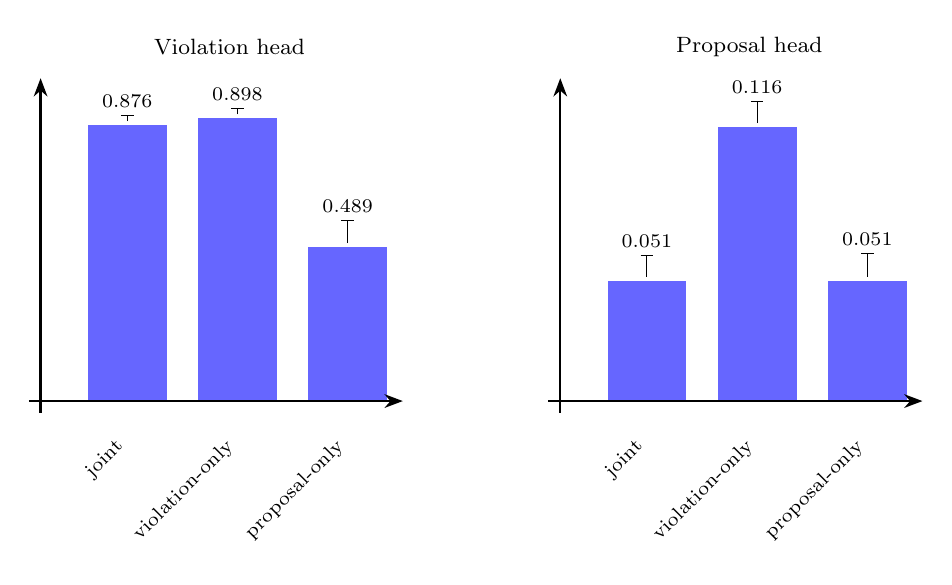
\begin{tikzpicture}[scale=1.0, transform shape]
  % Left panel: violation accuracy (joint 0.876, vio-only 0.898, prop-only 0.489)
  % scale: 1.0 = 4cm, y = value*4
  \def\sc{4}
  \begin{scope}[shift={(0,0)}]
    \node[font=\footnotesize] at (2.4,4.5) {Violation head};
    % joint
    \fill[blue!60] (0.6,0) rectangle (1.6,{0.876*\sc});
    % violation-only
    \fill[blue!60] (2.0,0) rectangle (3.0,{0.898*\sc});
    % proposal-only
    \fill[blue!60] (3.4,0) rectangle (4.4,{0.489*\sc});
    % error bars with caps (std: 0.019, 0.018, 0.071); labels above caps
    \draw (1.1,{0.876*\sc+0.05}) -- (1.1,{0.876*\sc+0.05+0.019*\sc});
    \draw (1.02,{0.876*\sc+0.05+0.019*\sc}) -- (1.18,{0.876*\sc+0.05+0.019*\sc});
    \node[font=\scriptsize] at (1.1,{0.876*\sc+0.05+0.019*\sc+0.18}) {0.876};
    \draw (2.5,{0.898*\sc+0.05}) -- (2.5,{0.898*\sc+0.05+0.018*\sc});
    \draw (2.42,{0.898*\sc+0.05+0.018*\sc}) -- (2.58,{0.898*\sc+0.05+0.018*\sc});
    \node[font=\scriptsize] at (2.5,{0.898*\sc+0.05+0.018*\sc+0.18}) {0.898};
    \draw (3.9,{0.489*\sc+0.05}) -- (3.9,{0.489*\sc+0.05+0.071*\sc});
    \draw (3.82,{0.489*\sc+0.05+0.071*\sc}) -- (3.98,{0.489*\sc+0.05+0.071*\sc});
    \node[font=\scriptsize] at (3.9,{0.489*\sc+0.05+0.071*\sc+0.18}) {0.489};
    \draw[thick,-{Stealth}] (0,-0.15) -- (0,4.1);
    \draw[thick,-{Stealth}] (-0.15,0) -- (4.6,0);
    \node[font=\scriptsize, rotate=45, anchor=east] at (1.1,-0.45) {joint};
    \node[font=\scriptsize, rotate=45, anchor=east] at (2.5,-0.45) {violation-only};
    \node[font=\scriptsize, rotate=45, anchor=east] at (3.9,-0.45) {proposal-only};
  \end{scope}
  % Right panel: proposal MSE (joint 0.051, vio-only 0.116, prop-only 0.051)
  % MSE scale: 1.0 = 30cm, y = value*30 (0.116 -> 3.48cm, matches left panel)
  \def\scm{30}
  \begin{scope}[shift={(6.6,0)}]
    \node[font=\footnotesize] at (2.4,4.5) {Proposal head};
    \fill[blue!60] (0.6,0) rectangle (1.6,{0.051*\scm});
    \fill[blue!60] (2.0,0) rectangle (3.0,{0.116*\scm});
    \fill[blue!60] (3.4,0) rectangle (4.4,{0.051*\scm});
    % error bars with caps (std: 0.009, 0.009, 0.010) *30; labels above caps
    \draw (1.1,{0.051*\scm+0.05}) -- (1.1,{0.051*\scm+0.05+0.009*\scm});
    \draw (1.02,{0.051*\scm+0.05+0.009*\scm}) -- (1.18,{0.051*\scm+0.05+0.009*\scm});
    \node[font=\scriptsize] at (1.1,{0.051*\scm+0.05+0.009*\scm+0.18}) {0.051};
    \draw (2.5,{0.116*\scm+0.05}) -- (2.5,{0.116*\scm+0.05+0.009*\scm});
    \draw (2.42,{0.116*\scm+0.05+0.009*\scm}) -- (2.58,{0.116*\scm+0.05+0.009*\scm});
    \node[font=\scriptsize] at (2.5,{0.116*\scm+0.05+0.009*\scm+0.18}) {0.116};
    \draw (3.9,{0.051*\scm+0.05}) -- (3.9,{0.051*\scm+0.05+0.010*\scm});
    \draw (3.82,{0.051*\scm+0.05+0.010*\scm}) -- (3.98,{0.051*\scm+0.05+0.010*\scm});
    \node[font=\scriptsize] at (3.9,{0.051*\scm+0.05+0.010*\scm+0.18}) {0.051};
    \draw[thick,-{Stealth}] (0,-0.15) -- (0,4.1);
    \draw[thick,-{Stealth}] (-0.15,0) -- (4.6,0);
    \node[font=\scriptsize, rotate=45, anchor=east] at (1.1,-0.45) {joint};
    \node[font=\scriptsize, rotate=45, anchor=east] at (2.5,-0.45) {violation-only};
    \node[font=\scriptsize, rotate=45, anchor=east] at (3.9,-0.45) {proposal-only};
  \end{scope}
\end{tikzpicture}
\caption{Training-objective ablation over 5 seeds (mean $\pm$ std): joint
training balances the two heads, while single-objective training degrades the
other head.}
\label{fig:phase9}
\end{figure}

\subsection{Element Completion}
We compare the GNN proposal head against a nearest-neighbor baseline that
copies the box of the closest surviving element (Fig.~\ref{fig:completion}).
At low drop ratios (0.2--0.4) the baseline wins because many survivors are
nearby. At high drop ratios (0.6--0.8) the GNN wins: at drop 0.6 the
GNN reaches IoU 0.122 vs.\ 0.088 for NN ($+39\%$); at drop 0.8, 0.097 vs.\
0.062 ($+56\%$). With fewer survivors, structural reasoning matters more than
proximity, which is consistent with the model using structural priors rather
than simple interpolation.

\begin{figure}[htbp]
\centering
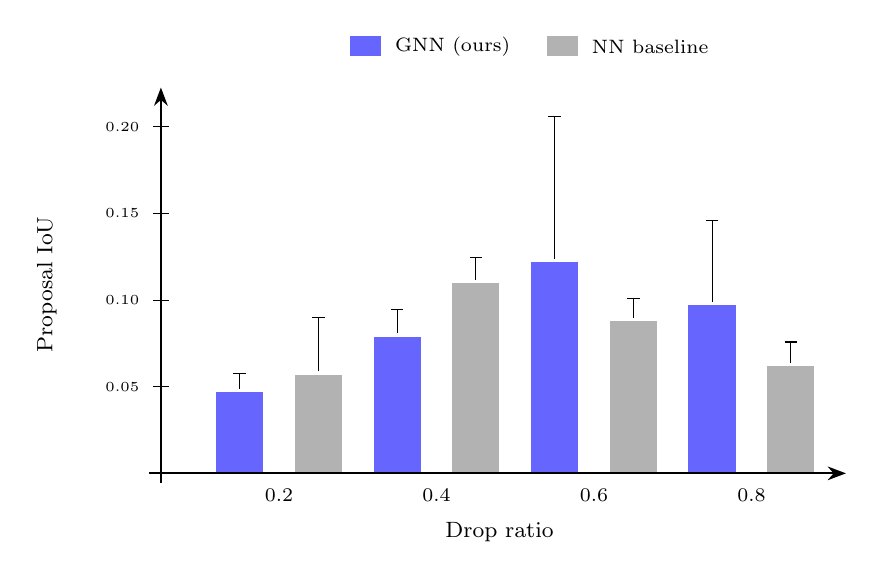
\begin{tikzpicture}[scale=1.0, transform shape]
  % grouped bars: 4 drop ratios x {GNN, NN}; y = value * 22 cm (max ~0.204 -> 4.5cm)
  \def\sc{22}
  % drop 0.2: GNN 0.047+/-0.009, NN 0.057+/-0.031
  % drop 0.4: GNN 0.079+/-0.014, NN 0.110+/-0.013
  % drop 0.6: GNN 0.122+/-0.082, NN 0.088+/-0.011
  % drop 0.8: GNN 0.097+/-0.047, NN 0.062+/-0.012
  % x positions: group i center at 1+2i, bars at center-0.3 and center+0.3
  \begin{scope}
    % legend (top center, above axis)
    \fill[blue!60] (2.4,5.3) rectangle (2.8,5.55);
    \node[anchor=west, font=\scriptsize] at (2.85,5.42) {GNN (ours)};
    \fill[gray!60] (4.9,5.3) rectangle (5.3,5.55);
    \node[anchor=west, font=\scriptsize] at (5.35,5.42) {NN baseline};
    % group 1: drop 0.2
    \fill[blue!60] (0.7,0) rectangle (1.3,{0.047*\sc});
    \draw (1.0,{0.047*\sc+0.04}) -- (1.0,{0.047*\sc+0.04+0.009*\sc});
    \draw (0.92,{0.047*\sc+0.04+0.009*\sc}) -- (1.08,{0.047*\sc+0.04+0.009*\sc});
    \fill[gray!60] (1.7,0) rectangle (2.3,{0.057*\sc});
    \draw (2.0,{0.057*\sc+0.04}) -- (2.0,{0.057*\sc+0.04+0.031*\sc});
    \draw (1.92,{0.057*\sc+0.04+0.031*\sc}) -- (2.08,{0.057*\sc+0.04+0.031*\sc});
    \node[font=\scriptsize] at (1.5,-0.28) {0.2};
    % group 2: drop 0.4
    \fill[blue!60] (2.7,0) rectangle (3.3,{0.079*\sc});
    \draw (3.0,{0.079*\sc+0.04}) -- (3.0,{0.079*\sc+0.04+0.014*\sc});
    \draw (2.92,{0.079*\sc+0.04+0.014*\sc}) -- (3.08,{0.079*\sc+0.04+0.014*\sc});
    \fill[gray!60] (3.7,0) rectangle (4.3,{0.110*\sc});
    \draw (4.0,{0.110*\sc+0.04}) -- (4.0,{0.110*\sc+0.04+0.013*\sc});
    \draw (3.92,{0.110*\sc+0.04+0.013*\sc}) -- (4.08,{0.110*\sc+0.04+0.013*\sc});
    \node[font=\scriptsize] at (3.5,-0.28) {0.4};
    % group 3: drop 0.6
    \fill[blue!60] (4.7,0) rectangle (5.3,{0.122*\sc});
    \draw (5.0,{0.122*\sc+0.04}) -- (5.0,{0.122*\sc+0.04+0.082*\sc});
    \draw (4.92,{0.122*\sc+0.04+0.082*\sc}) -- (5.08,{0.122*\sc+0.04+0.082*\sc});
    \fill[gray!60] (5.7,0) rectangle (6.3,{0.088*\sc});
    \draw (6.0,{0.088*\sc+0.04}) -- (6.0,{0.088*\sc+0.04+0.011*\sc});
    \draw (5.92,{0.088*\sc+0.04+0.011*\sc}) -- (6.08,{0.088*\sc+0.04+0.011*\sc});
    \node[font=\scriptsize] at (5.5,-0.28) {0.6};
    % group 4: drop 0.8
    \fill[blue!60] (6.7,0) rectangle (7.3,{0.097*\sc});
    \draw (7.0,{0.097*\sc+0.04}) -- (7.0,{0.097*\sc+0.04+0.047*\sc});
    \draw (6.92,{0.097*\sc+0.04+0.047*\sc}) -- (7.08,{0.097*\sc+0.04+0.047*\sc});
    \fill[gray!60] (7.7,0) rectangle (8.3,{0.062*\sc});
    \draw (8.0,{0.062*\sc+0.04}) -- (8.0,{0.062*\sc+0.04+0.012*\sc});
    \draw (7.92,{0.062*\sc+0.04+0.012*\sc}) -- (8.08,{0.062*\sc+0.04+0.012*\sc});
    \node[font=\scriptsize] at (7.5,-0.28) {0.8};
    % axes
    \draw[thick,-{Stealth}] (0,-0.12) -- (0,4.9);
    \draw[thick,-{Stealth}] (-0.15,0) -- (8.7,0);
    \node[font=\footnotesize] at (4.3,-0.75) {Drop ratio};
    \node[font=\footnotesize, rotate=90] at (-1.45,2.4) {Proposal IoU};
    \foreach \v in {0.05,0.10,0.15,0.20} {
      \draw (-0.1,{\v*\sc}) -- (0.1,{\v*\sc});
      \node[anchor=east, font=\tiny] at (-0.15,{\v*\sc}) {\v};
    }
  \end{scope}
\end{tikzpicture}
\caption{Element-completion IoU vs.\ drop ratio (mean $\pm$ std, 2 seeds).
The GNN beats the nearest-neighbor baseline when substantial structure is
missing (drop 0.6--0.8).}
\label{fig:completion}
\end{figure}

\subsection{End-to-End on Real VLM Output}
We deploy the trained model behind Qwen3-VL Flash on 200 real RICO
screenshots (4789 ground-truth elements, 2947 VLM predictions). The GNN
receives the VLM's noisy elements, detects violated constraints, and proposes
missing elements; proposals are merged with non-maximum suppression. We
evaluate with center-distance matching at threshold 0.1 against ground truth
(Table~\ref{tab:real}, Fig.~\ref{fig:realvlm}).

\begin{table}[htbp]
\caption{End-to-end results on 200 real RICO screenshots (pooled).
Checkpoints loaded with shape-filtering; numbers reflect correctly loaded
weights.}
\label{tab:real}
\centering
\begin{tabularx}{\textwidth}{Xccc}
\toprule
\textbf{Metric} & \textbf{VLM only} & \textbf{VLM + GNN} & \textbf{$\Delta$} \\
\midrule
Precision & 0.382 & 0.393 & $+1.1$pp \\
Recall & 0.235 & 0.257 & $+2.2$pp \\
F1 & 0.291 & 0.311 & $+2.0$pp \\
TP / FP / FN & 1126/1821/3663 & 1232/1905/3557 & $+106$ TP \\
\bottomrule
\end{tabularx}
\end{table}

\begin{figure}[htbp]
\centering
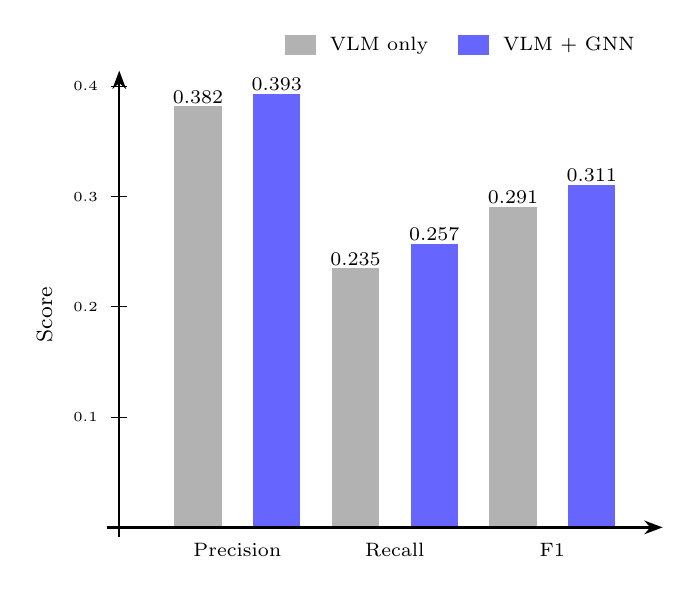
\begin{tikzpicture}[scale=1.0, transform shape]
  % before/after: Precision 0.382->0.393, Recall 0.235->0.257, F1 0.291->0.311
  % y = value * 14 cm (0.393 -> 5.5cm); axis top 6.2 to leave room for labels
  \def\sc{14}
  % legend (top center, above axis)
  \fill[gray!60] (2.1,6.0) rectangle (2.5,6.25);
  \node[anchor=west, font=\scriptsize] at (2.55,6.12) {VLM only};
  \fill[blue!60] (4.3,6.0) rectangle (4.7,6.25);
  \node[anchor=west, font=\scriptsize] at (4.75,6.12) {VLM + GNN};
  % Precision
  \fill[gray!60] (0.7,0) rectangle (1.3,{0.382*\sc});
  \node[font=\scriptsize] at (1.0,{0.382*\sc+0.12}) {0.382};
  \fill[blue!60] (1.7,0) rectangle (2.3,{0.393*\sc});
  \node[font=\scriptsize] at (2.0,{0.393*\sc+0.12}) {0.393};
  \node[font=\scriptsize] at (1.5,-0.28) {Precision};
  % Recall
  \fill[gray!60] (2.7,0) rectangle (3.3,{0.235*\sc});
  \node[font=\scriptsize] at (3.0,{0.235*\sc+0.12}) {0.235};
  \fill[blue!60] (3.7,0) rectangle (4.3,{0.257*\sc});
  \node[font=\scriptsize] at (4.0,{0.257*\sc+0.12}) {0.257};
  \node[font=\scriptsize] at (3.5,-0.28) {Recall};
  % F1
  \fill[gray!60] (4.7,0) rectangle (5.3,{0.291*\sc});
  \node[font=\scriptsize] at (5.0,{0.291*\sc+0.12}) {0.291};
  \fill[blue!60] (5.7,0) rectangle (6.3,{0.311*\sc});
  \node[font=\scriptsize] at (6.0,{0.311*\sc+0.12}) {0.311};
  \node[font=\scriptsize] at (5.5,-0.28) {F1};
  % axes
  \draw[thick,-{Stealth}] (0,-0.12) -- (0,5.8);
  \draw[thick,-{Stealth}] (-0.15,0) -- (6.9,0);
  \node[font=\footnotesize, rotate=90] at (-0.95,2.7) {Score};
  \foreach \v in {0.1,0.2,0.3,0.4} {
    \draw (-0.1,{\v*\sc}) -- (0.1,{\v*\sc});
    \node[anchor=east, font=\tiny] at (-0.15,{\v*\sc}) {\v};
  }
\end{tikzpicture}
\caption{End-to-end: VLM only vs.\ VLM + GNN (corrected checkpoint loading).
Recall and F1 improve while precision also rises slightly.}
\label{fig:realvlm}
\end{figure}

The corrected pipeline recovers 106 previously missed elements ($+106$ TP,
$+2.2$pp recall) at a cost of 84 additional false positives, improving F1 by
2.0 points. Precision also improves slightly ($+1.1$pp), unlike earlier
results reported with incorrectly loaded checkpoints, a subtle but
important evaluation pitfall. An earlier evaluation loaded a checkpoint with
mismatched hidden dimensions under non-strict weight loading, silently
dropping 89\% of the weights and producing a spurious $+2.9$pp F1 gain from
near-random weights. All results reported here use shape-filtered checkpoint
loading, which only keeps weights whose shapes match, and we recommend this
as a standard practice.

\subsection{Performance}
The correction network is small (57K parameters). Graph construction takes
about 5~ms and inference about 0.53~ms (p50) per screenshot on a CPU-only
M3 MacBook Pro, negligible compared with VLM inference at roughly two seconds
per image. Training 2,000 samples $\times$ 50 epochs completes in under five
minutes on CPU.

\section{Discussion}
\subsection{When Does Structural Reasoning Help?}
Across the experiments, structural reasoning helped most when the VLM output
was sparse (many elements missing) and less when the VLM was already
accurate. This mirrors the sequence of negative results that motivated the
graph formulation in the first place. On simulated Gaussian noise, the model
never beat the no-op baseline; Qwen3-VL Plus and Flash produced positional
errors around 0.01 or smaller, leaving nothing to correct; LLaVA-7B detected
only a few elements per screenshot, so the graph carried little structure;
and a reweighted existence-only objective had no false positives to filter.
Only when a substantial fraction of elements was missing did the constraint
graph contain information that a per-element regressor could not access. For
lightweight VLMs on realistic screenshots (which omit 10--30\% of elements),
this regime is the relevant one for practical use.

\subsection{Limitations}
The main limitations are as follows. First, \emph{type prediction is weak}: predicting
an element's semantic type from constraint context alone caps at 62\%
accuracy; constraints carry spatial but not semantic information. Second,
\emph{domain transfer is limited}: the confidence model's AUROC drops from
0.703 on RICO to 0.554 on ScreenSpot, indicating that false-positive patterns
learned on mobile screens do not fully transfer to mixed mobile/PC/web
layouts. Third, \emph{dense toolbars are hard}: a toolbar with 8+ tiny icons
creates a dense constraint graph in which individual elements are hard to
distinguish, and free-form layouts (maps, drawings) offer few constraints to
reason from.

\subsection{Future Work}
Visual feature fusion with cross-attention is a candidate next step (early
experiments show 18--22\% proposal-MSE improvement), as is domain adaptation
to ScreenSpot. Extending the graph with temporal context could help the model
distinguish missing elements from elements hidden by UI state.

\section{Conclusion}
This report presented a heterogeneous bipartite GraphSAGE framework for
correcting noisy GUI element predictions from lightweight VLMs. Ten spatial
constraint types are encoded as a bipartite graph, so elements exchange
messages only through shared constraints; the multi-task objective couples
coordinate correction, violation detection, existence scoring, and
self-supervised element completion. On RICO, the model achieves 90--94\%
violation accuracy, a $+56\%$ IoU gain over nearest-neighbor completion at
high drop ratios, and a $+2.0$pp F1 improvement on 200 real Qwen3-VL Flash
screenshots with shape-filtered checkpoint loading.

The results are encouraging but bounded. The gains appear when the VLM output
is sparse, and the framework inherits the VLM's initial detections; it does
not fix errors that are purely semantic, and its confidence scores transfer
only partially across domains. These limits, along with the negative results
reported in the discussion, suggest that structural post-correction is best
viewed as one component of a GUI-understanding pipeline rather than a
complete solution. Whether the approach generalizes beyond mobile layouts to
desktop and web interfaces remains to be tested.

\section*{Acknowledgment}
The author thanks Prof.\ Wing Cheong Lau for supervision and guidance
throughout the internship, and the CUHK Information Engineering Department
for support.

\bibliographystyle{unsrtnat}
\bibliography{references}

\end{document}
